\subsection{Restrições}
% Requested

Devido à simplicidade do problema, este não contém restrições flexíveis, apenas restrições rígidas, tanto para os operadores como para os operandos.

% -----------------

\subsubsection{Operadores} No predicado \verb|operators(1,_,_)| é criada uma lista de operadores que pode ser alimentada ao predicado \verb|gold_star/2|. Nesta criação é aplicada uma restrição explicita no predicado \verb|bigger/2|:

\begin{proof}
O primeiro operador de uma configuração deve ter maior ou igual valor numérico que os restantes operadores
\end{proof}

\begin{figure}[h]
\centering
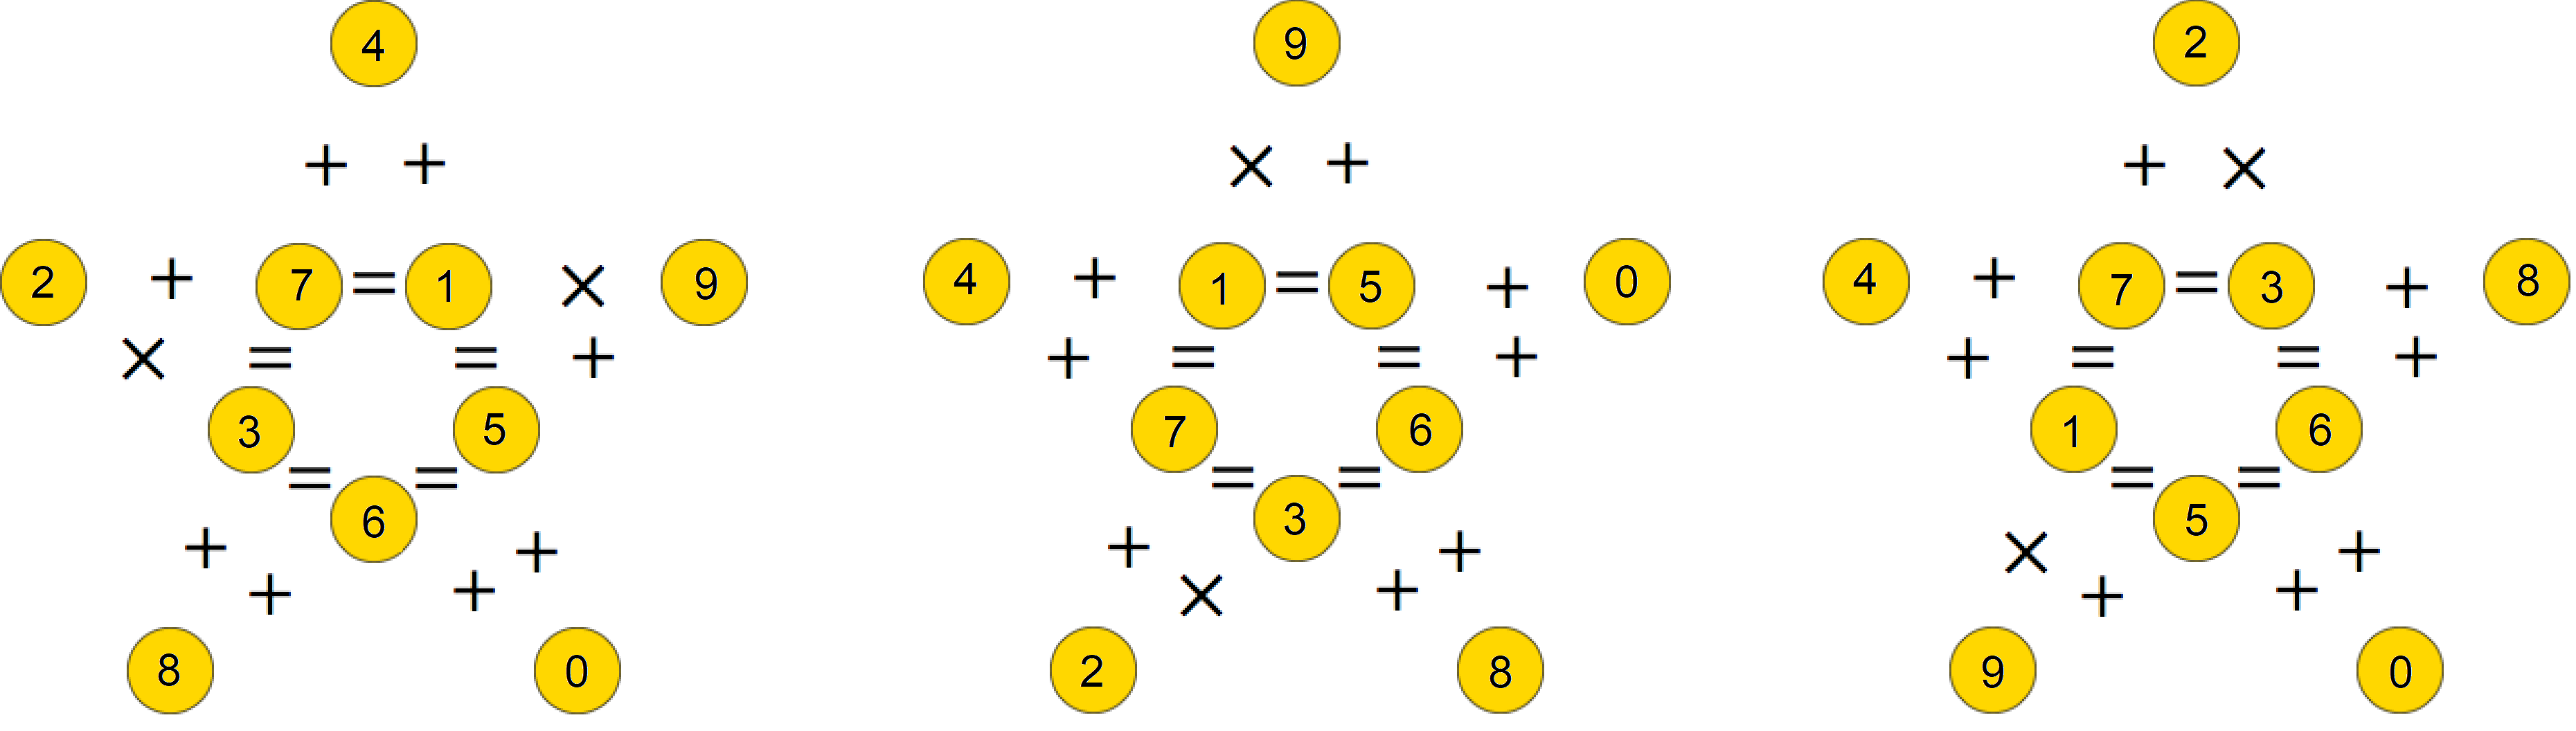
\includegraphics[width=\textwidth]{figuras/rotated.png}
\caption{A estrela do centro tem a configuração [3,1,1,1,1,1,3,1,1,1]. A estrela da esquerda é obtida através de uma rotação da estrela do centro, formando a configuração [1,1,3,1,1,1,1,1,3,1]. A estrela da direita é obtida através de uma combinação de uma rotação e uma reflexão, resultando na configuração [1,3,1,1,1,1,1,3,1,1]}
\label{fig: ops_restriction}
\end{figure}

Na figura \ref{fig: ops_restriction} apenas a configuração central obedece à restrição e só essa configuração é calculada. Todas as outras configurações, possíveis de obter através de deslocamentos de todos os elementos dentro da lista correspondem a aplicar rotações e reflexões na estrela original, o que faz com que seja desnecessário calcular estas configurações, já que são facilmente obtidas.

\begin{figure}
    \centering
    \begin{tabular}{c}
    \begin{lstlisting}[language=Prolog]
    bigger(_, []).
    bigger(Op1, [Op | Rest]) :-
        Op1 #>= Op,
        bigger(Op1, Rest).
    \end{lstlisting}
    \end{tabular}
    \caption{Predicado bigger/2 que recebe como primeiro argumento o primeiro elemento da lista a ser instanciado, e aplica a restrição \#>= a todos os restantes elementos. A condição termina quando não houver mais operadores á qual se possa aplicar a restrição}
    \label{code:bigger}
\end{figure}

% -----------------

\subsubsection{Operandos} Na primeira fase do projeto só era possível solucionar uma estrela de cinco pontas. Isto facilitou a aplicação de restrições, já que as únicas restrições que eram necessárias correspondiam ás equações da estrela (Fig. \ref{code:predicados_restricoes}).

Com a adição de funcionalidade dimensional foi necessário refazer os predicados que atribuíam as restrições aos operadores. Verificou-se que, da forma como os operandos e os operadores são declarados \footnote{Os operadores são declarados, começando no ponta do topo, primeiro o operador da esquerda, depois o da direita, continua-se no sentido horário para as outras pontas. Os operandos são declarados, começando no operador do topo da estrela, em sentido horário, passando para a base da próxima ponta, depois para o topo da ponta e continua até acabar.} era possível achar uma forma de declarar restrições de forma iterativa.

Para saber as equações que resultavam de uma estrela de n pontas era necessário desenhar a estrela e ver as equações uma a uma analisando cada ponta da estrela. Com o método achado, é possível criar um conjunto de \enquote{equações direccionais} a partir de um tamanho de pontas e retirar facilmente daí o conjunto de equações.

Para criar um conjunto de equações direccionais a partir de um número de pontas, começa-se por definir a primeira e as duas últimas equações, já que estas são semelhantes para qualquer número de pontas. Estas equações são lidas da esquerda para a direita. As restantes equações (excepto para a estrela de 3 pontas que apenas possui 3 equações) são formadas usando os restantes operadores e operandos de acordo com a figura \ref{fig: restriction_method}, lidas da direita para a esquerda. A ordem de leitura importa devido aos operadores - e ÷ que não são comutativos.

Este método traduz-se para prolog a partir dos predicados \verb^first_restrictions/2^ e \verb#remaining_restrictions/2#. No primeiro predicado são declaradas as restrições que correspondem às 3 equações comuns a todos e no segundo predicado são aplicadas iterativamente o resto das restrições.
